\section{Resultados}
\subsection{Reconstrucción histórica y comparación original}\label{sec:historical-loss}
La auditoría histórica preservó 1720 archivos físicos de predicciones:1240 mediante integridad y 480 compactos mediante recomputación. Las 337120 filas físicas excluyen 23520 filas adicionales del alias V2. Treinta estados finales entrenados coincidieron con referencias archivadas. La discrepancia máxima agregada MASE de $4.66\times 10^{-10}$ se conservó como precisión numérica, no como mejora por entrenamiento. Los pilotos previos usaban otra partición; aquí se utiliza la versión 70/10/20 realmente ejecutada.

La Tabla~\ref{tab:historical-main} reúne las seis condiciones con pérdidas sobre 28 servicios. E5 obtuvo CPU MASE1.002387 frente a 0.992620 de E0, y memoria 1.121358 frente a 1.135901. Las reducciones emparejadas por máscara son $-0.984\%$ y $1.280\%$, respectivamente. GRU de llamadas presentó CPU MASE0.939410, el menor histórico mostrado, sin demostrar superioridad general del grafo. GinAR conservó CPU MASE280825.103210, resultado extremo de esta implementación y presupuesto. La verificación no justificó excluirlo ni atribuirlo al comportamiento general del método publicado.
\begin{table*}[!t]
\caption{Promedios históricos de seis condiciones con pérdidas, 28 servicios, tres semillas neuronales y veinte máscaras. Los errores absolutos CPU conservan escala publicada; memoria se expresa en bytes. V2 es un alias seleccionado.}\label{tab:historical-main}
\centering\footnotesize
\FitTable{\begin{tabular}{lrrrrrr}
\toprule
Modelo & CPU MASE & CPU MAE & CPU RMSE & Mem. MASE & Mem. MAE & Mem. RMSE \\
\midrule
persistencia & 1.07741 & 0.000300957 & 0.000505471 & 1.31287 & 1.30725e+06 & 2.01898e+06 \\
E0 & 0.99262 & 0.000302127 & 0.000456189 & 1.1359 & 1.10867e+06 & 1.694e+06 \\
E1 & 1.02275 & 0.000307441 & 0.000457202 & 1.1359 & 1.10867e+06 & 1.694e+06 \\
E2 & 1.02163 & 0.000305333 & 0.000453692 & 1.12503 & 1.09644e+06 & 1.6773e+06 \\
E3 & 1.00514 & 0.000304111 & 0.000455915 & 1.1345 & 1.10712e+06 & 1.69482e+06 \\
E4 & 0.98954 & 0.000301872 & 0.000456377 & 1.13528 & 1.10705e+06 & 1.69286e+06 \\
E5 & 1.00239 & 0.000305151 & 0.000455849 & 1.12136 & 1.0933e+06 & 1.67625e+06 \\
C0 & 1.02163 & 0.000305333 & 0.000453692 & 1.1359 & 1.10867e+06 & 1.694e+06 \\
C1 & 1.02095 & 0.000305271 & 0.000453709 & 1.1351 & 1.10785e+06 & 1.69341e+06 \\
C2 & 1.02151 & 0.000305326 & 0.000453707 & 1.13576 & 1.10848e+06 & 1.69381e+06 \\
C3 & 1.02092 & 0.000305271 & 0.000453723 & 1.13522 & 1.10794e+06 & 1.69342e+06 \\
V2 & 1.02092 & 0.000305271 & 0.000453723 & 1.1351 & 1.10785e+06 & 1.69341e+06 \\
GRU\_propia & 0.955358 & 0.000279717 & 0.0004371 & 1.16785 & 1.15154e+06 & 1.76786e+06 \\
GRU\_llamadas & 0.93941 & 0.000274958 & 0.000430716 & 1.19984 & 1.18269e+06 & 1.81389e+06 \\
BiTGraph\_codigo\_autor & 1.00373 & 0.000282931 & 0.000428389 & 1.21558 & 1.18535e+06 & 1.79317e+06 \\
GinAR & 280825 & 63.2538 & 1254.57 & 2.5045 & 2.27786e+06 & 4.49626e+06 \\
\bottomrule
\end{tabular}}
\end{table*}

Dentro de E0--E5, E2 mejoró memoria a 1.125032, pero empeoró CPU a 1.021630. E4 tuvo el menor CPU MASE entre esas seis variantes, 0.989540, con memoria 1.135284. E1 y E3 no mejoraron ambos recursos. E5 no representa una acumulación monótona de ganancias. La mejora adicional emparejada de memoria frente a E2 fue aproximadamente 0.327\%, con más parámetros y mayor coste medido. Las configuraciones seleccionadas no aíslan efectos causales de cada componente.

\subsection{Familias compactas C, V2 e incertidumbre histórica}\label{sec:historical-compact}
Los MASE CPU de C0--C3 fueron 1.021630, 1.020946, 1.021505 y 1.020919; en memoria, 1.135901, 1.135097, 1.135755 y 1.135218. V2 seleccionó C3/EMA0.7 para CPU y C1/MA25 para memoria con validación media 0.911214 y 0.998329. La prueba resultó 1.020919/1.135097 y reducciones $-2.851\%$/$0.071\%$ contra E0. Contra E5 las reducciones fueron $-1.849\%$/$-1.225\%$. La simplificación no conservó toda la ventaja histórica de memoria ni mejoró conjuntamente frente a E0.

Los intervalos de diferencia E5 condicionados solo a máscaras fueron $[-0.010137,\allowbreak -0.009395]$ en CPU y $[0.014296,\allowbreak 0.014793]$ en memoria. Al cruzar semillas y máscaras se ampliaron a $[-0.028165,\allowbreak 0.026164]$ y \allowbreak $[-0.002967,\allowbreak 0.024027]$, ambos incluyendo cero. Una de tres semillas favoreció E5 en CPU y dos de tres en memoria. Aunque los 28 promedios de servicio de memoria favorecieron E5, comparten período y relaciones; no son 28 ensayos independientes. Los intervalos estrechos condicionales no demuestran estabilidad entre organizaciones ni inicializaciones arbitrarias.

Las curvas históricas mostradas de E0/E2/E4/E5/V2 aumentaron con 0, 10, 20 y 40\% bajo ambos patrones y recursos: veinte curvas crecientes, no una propiedad de todos los comparadores o series. El benchmark CUDA B128 registró p 50 CPU de 0.284/0.814/0.691~ms para E0/E5/V2 y memoria 0.287/0.801/0.416~ms. V2 tiene 28/27 parámetros, frente a 74 de E5, pero su ejecución CPU siguió siendo más lenta que E0. Estas mediciones históricas de diez calentamientos no se mezclan con B1 ampliado de veinte calentamientos. Las Figs.~\ref{fig:historical} y~\ref{fig:evolution} muestran comparación y evolución conceptual.
\begin{figure*}[!t]\centering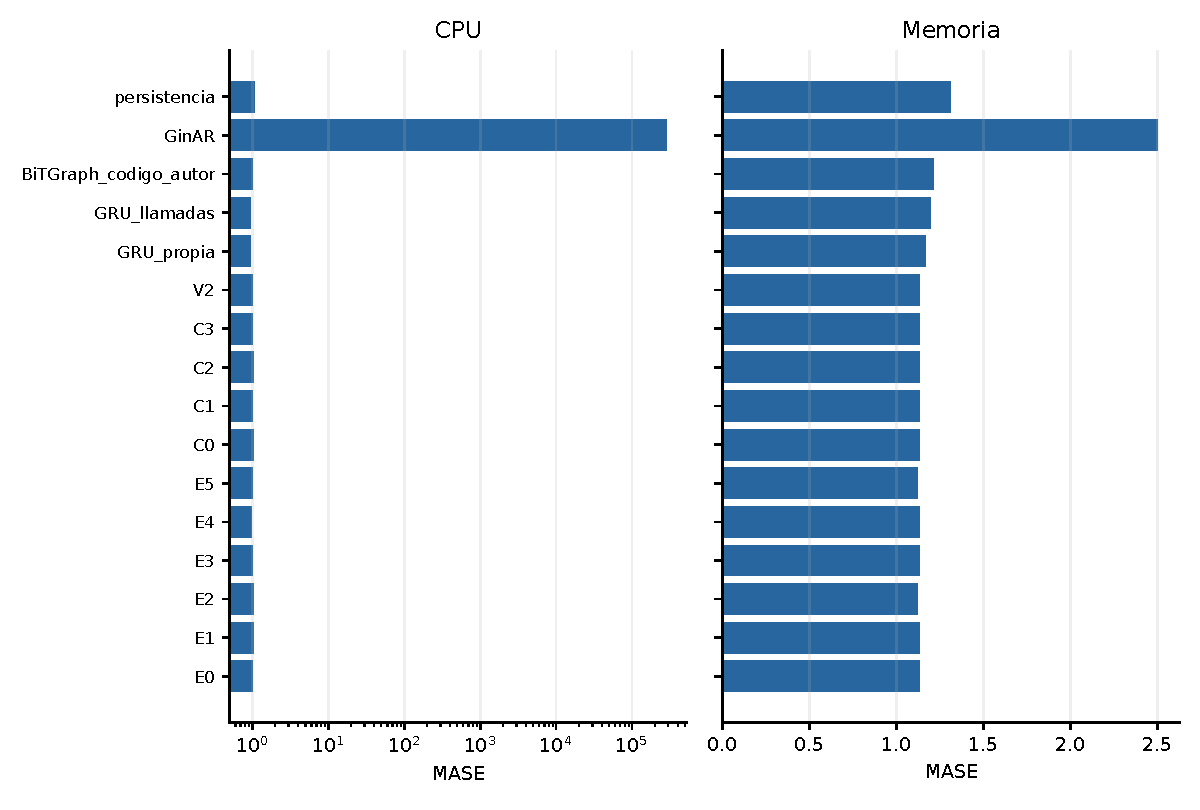
\includegraphics[width=0.82\textwidth]{figuras/es_historico.pdf}
\caption{MASE histórico de seis condiciones con pérdidas. La escala logarítmica CPU conserva el extremo de GinAR; memoria utiliza escala lineal. Son resultados fuente 28.}\label{fig:historical}\end{figure*}
\begin{figure*}[!t]\centering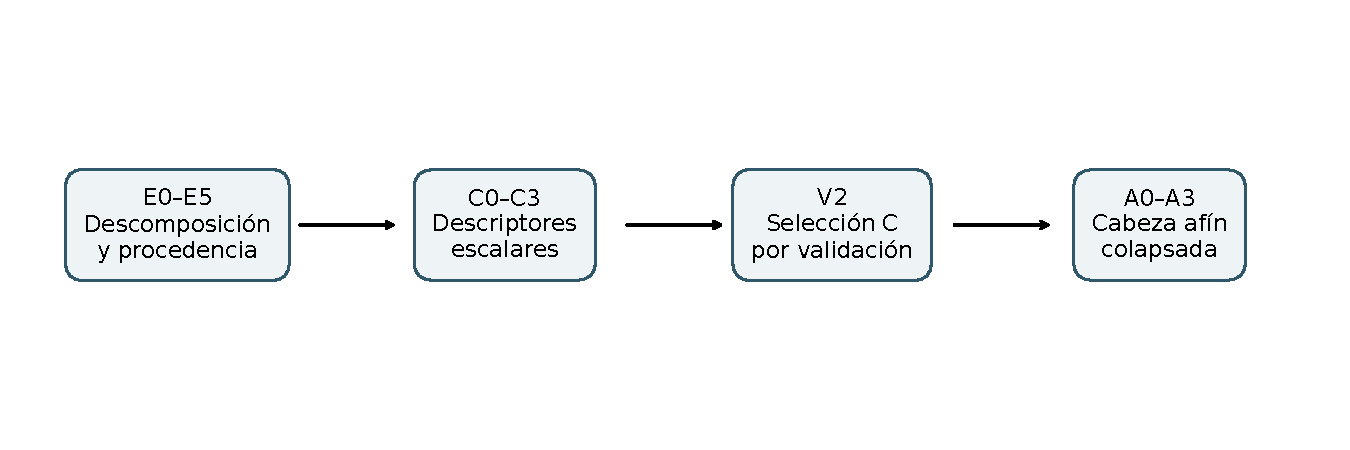
\includegraphics[width=0.91\textwidth]{figuras/es_evolucion.pdf}
\caption{E cambia descomposición o descriptores completos; C mantiene dos cabezas con descriptores escalares; V2 selecciona ajustes C existentes; A colapsa la proyección afín fija. Las flechas indican orden de estudio, sin garantizar mejoras.}\label{fig:evolution}\end{figure*}

\subsection{Finalización ampliada, integridad y pérdidas realizadas}\label{sec:completion}
Se completaron L12/H1, seis configuraciones secundarias y transferencia externa con pesos congelados:364 ajustes neuronales finales, 56 registros simples por configuración/recurso y 280 ajustes cortos fuente. Se guardaron 9680 archivos de predicciones y 3097600 filas de métricas por servicio. La reconstrucción independiente float 64 comprobó índices, cantidades de objetivos, resúmenes criptográficos y MAE/RMSE/MASE desde todos los archivos. La discrepancia absoluta máxima fue $3.73\times 10^{-9}$ en unidades originales. Los 420 checkpoints finales y hashes fuente pasaron la auditoría. Las filas reiteran modelos, máscaras, semillas, servicios y condiciones; no representan datasets independientes.

Con etiqueta 20\%, los cuatro mecanismos de conteo exacto produjeron 19.988\% de ausencia inducida en la prueba ChronoGraph. MAR dependiente del retardo promedió 26.301\%, con rango 25.925--26.577\% entre veinte máscaras. En Alibaba el redondeo dio 20.833\% para conteo exacto y MAR 27.861\%, rango 26.042--30.469\%. La ausencia natural se registra aparte. El corte 70/10/20 corresponde a filas ChronoGraph; Alibaba contiene 12 intervalos de calibración y 36 objetivos.

\subsection{Comparación principal sobre 32 servicios}
La Tabla~\ref{tab:primary} y la Fig.~\ref{fig:models} presentan L12/H1 y seis condiciones originales con pérdidas. PatchTST tuvo los menores promedios MASE observados:1.0419 CPU y 1.2170 memoria; NLinear quedó cerca con 1.0463 y 1.2197. No se preespecificó una prueba confirmatoria entre ambos. La media móvil obtuvo CPU 1.0678, menor que DLinear 1.1493, E5 1.1454 y A3 1.1602. En memoria A0 fue la menor variante afín compacta, 1.2334; A3 obtuvo 1.2403, DLinear 1.2402 y E5 1.2656. Los dos coeficientes de ausencia no mejoraron el agregado A3 frente a A0. El beneficio histórico de E5 en memoria no se conservó como victoria sobre DLinear. GRU de grafo alcanzó memoria 1.4851; ninguna familia se eliminó por mal resultado.
\begin{table*}[!t]
\caption{Principal destino 32: ponderación igual de servicios, seis condiciones con pérdidas, máscaras y ajustes. MAE/RMSE CPU se muestran en $10^{-3}$ de escala publicada y memoria en MiB,$2^{20}$ bytes. MASE es adimensional. El rango no constituye significación.}\label{tab:primary}
\centering\footnotesize
\FitTable{\begin{tabular}{lrrrrrr}
\toprule
Modelo & CPU MASE & CPU MAE & CPU RMSE & Mem. MASE & Mem. MAE & Mem. RMSE \\
\midrule
Persistencia & 1.1170 & 3.3236 & 4.5878 & 1.2861 & 2.0009 & 3.3833 \\
Media móvil & 1.0678 & 2.9643 & 4.2038 & 1.2361 & 1.8956 & 3.2699 \\
Suavizamiento exponencial & 1.0691 & 2.8926 & 4.0646 & 1.2535 & 1.9130 & 3.2673 \\
Ridge & 1.2669 & 3.1952 & 4.3079 & 1.3613 & 1.9589 & 3.1848 \\
DLinear & 1.1493 & 2.9924 & 4.1015 & 1.2402 & 1.8762 & 3.1573 \\
NLinear & 1.0463 & 2.8499 & 3.9969 & 1.2197 & 1.8482 & 3.1422 \\
E5 & 1.1454 & 3.0142 & 4.1411 & 1.2656 & 1.9044 & 3.1560 \\
A0 & 1.1562 & 3.0028 & 4.1185 & 1.2334 & 1.8649 & 3.1605 \\
A1 & 1.1547 & 2.9986 & 4.1147 & 1.2397 & 1.8704 & 3.1591 \\
A2 & 1.1563 & 3.0030 & 4.1185 & 1.2443 & 1.8773 & 3.1650 \\
A3 & 1.1602 & 3.0095 & 4.1248 & 1.2403 & 1.8733 & 3.1629 \\
GRU (propia) & 1.2198 & 3.2253 & 4.5667 & 1.3438 & 2.1652 & 3.7094 \\
GRU (grafo) & 1.1949 & 3.2375 & 4.5153 & 1.4851 & 2.2017 & 3.6563 \\
GRU-D adaptada & 1.1766 & 3.1392 & 4.4427 & 1.3605 & 2.1647 & 3.6811 \\
PatchTST (pequeño) & 1.0419 & 2.8539 & 4.1061 & 1.2170 & 1.8649 & 3.1655 \\
\bottomrule
\end{tabular}
}
\end{table*}
\begin{figure*}[!t]\centering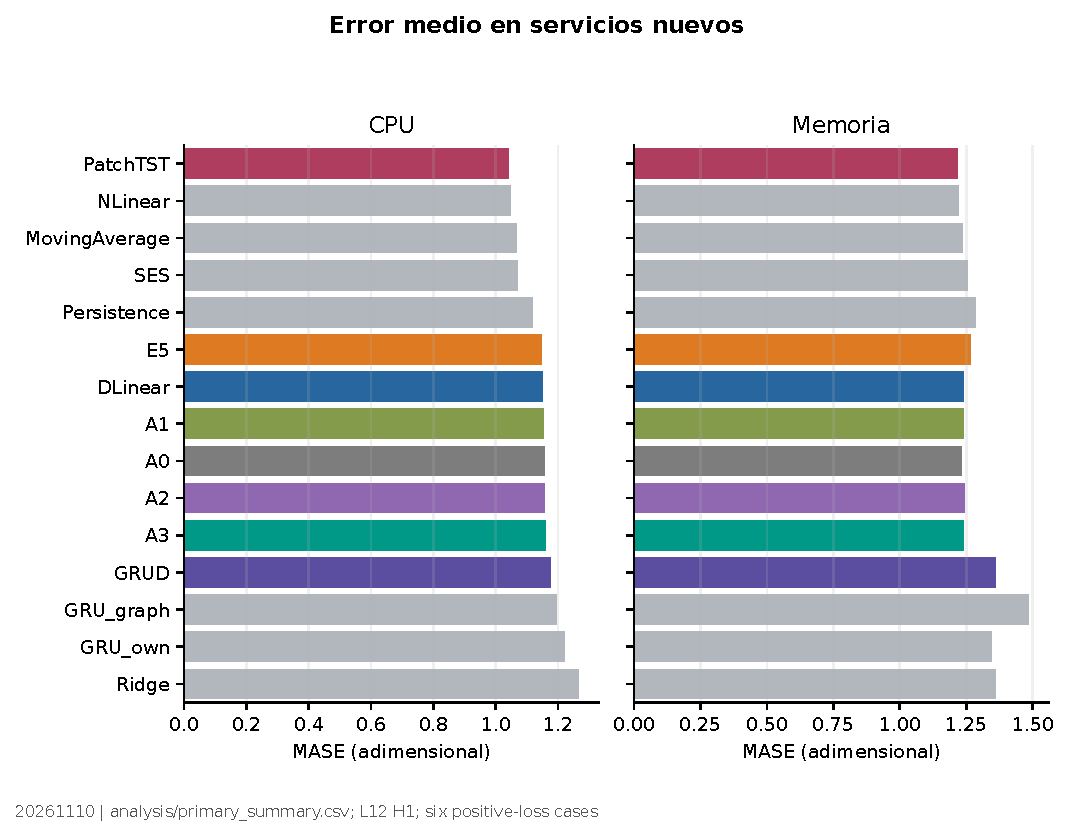
\includegraphics[width=0.79\textwidth]{figuras/es_06_models.pdf}
\caption{MASE principal de quince familias. La ordenación CPU solo organiza la presentación. Comparten servicios, máscaras y objetivos; se conserva la variación entre ajustes neuronales.}\label{fig:models}\end{figure*}

\subsection{Cuatro contrastes preespecificados y evaluación de A3}\label{sec:contrasts}
La Tabla~\ref{tab:contrasts} distingue diferencia media MASE y reducción media por celda. El único contraste con diez de diez semillas favorables fue A3 contra E5 en memoria:$\Delta=0.02523$, prueba bilateral exacta de signos ajustada Holm $ p=0.0078125$, intervalo condicional cruzado con bloques 48$[0.01312,\allowbreak 0.03981]$. La reducción media emparejada por celda fue 1.00\%; el cociente de medias da 1.99\%, otro estimando. Excluir la semilla de búsqueda 101 dejó nueve de nueve favorables y $ p=0.015625$ diagnóstico ajustado separadamente. Estos valores están condicionados a servicios, máscaras y período fijos, sin demostrar mejora de una población de sistemas.

Frente a DLinear, A3 tuvo $\Delta=-0.01090$ en CPU y $-0.00014$ en memoria, ambos $ p $ ajustada 1. Contra E5 en CPU,$\Delta=-0.01485$ y $ p=1$. Su intervalo temporal condicional excluye cero hacia valores negativos, mientras solo tres de diez semillas favorecen A3 y la prueba principal no rechaza. Los procedimientos tienen estimandos y supuestos diferentes; el intervalo no reemplaza la regla de cuatro pruebas. La Tabla~\ref{tab:block} presenta sensibilidad a bloques de 24, 48 y 96 pasos.
\begin{table*}[!t]
\caption{Contrastes principales:$\Delta=MASE_{referencia}-MASE_{A3}$. Positivo favorece A3. La media $ R $ promedia porcentajes de celdas, no cocientes globales. Los intervalos condicionan servicios fijos; las pruebas usan dirección de medias por semilla y Holm.}\label{tab:contrasts}
\centering\footnotesize
\FitTable{\begin{tabular}{lrrrrrr}
\toprule
Recurso & Referencia & $\Delta$MASE & Media $R$ (\%) & Condicional95\% interval & $p_{\mathrm{Holm}}$ & Semillas favorables \\
\midrule
CPU & DLinear & -0.01090 & -0.78 & [-0.02732, 0.00470] & 1 & 4/10 \\
CPU & E5 & -0.01485 & -1.95 & [-0.02977, -0.00120] & 1 & 3/10 \\
Memoria & DLinear & -0.00014 & 0.00 & [-0.00959, 0.01035] & 1 & 3/10 \\
Memoria & E5 & 0.02523 & 1.00 & [0.01312, 0.03981] & 0.007812 & 10/10 \\
\bottomrule
\end{tabular}
}
\end{table*}

La ventaja de memoria frente a E5 es heterogénea: favorece solo 10 de 32 servicios; service 540 aporta 42.4\% de la media. Excluirlo después de observar resultados deja $\Delta=0.01499$; excluir los tres servicios más favorables deja 0.00325 y seis de diez semillas favorables. Son exclusiones informadas por resultados, no análisis confirmatorios. La Fig.~\ref{fig:services} muestra los efectos por servicio predefinidos frente a DLinear. La Fig.~\ref{fig:ablation} conserva A0--A3 y la Fig.~\ref{fig:seeds} separa ajustes. Las máscaras repiten evaluación de los mismos pesos; no añaden entrenamientos independientes.
\begin{figure*}[!t]\centering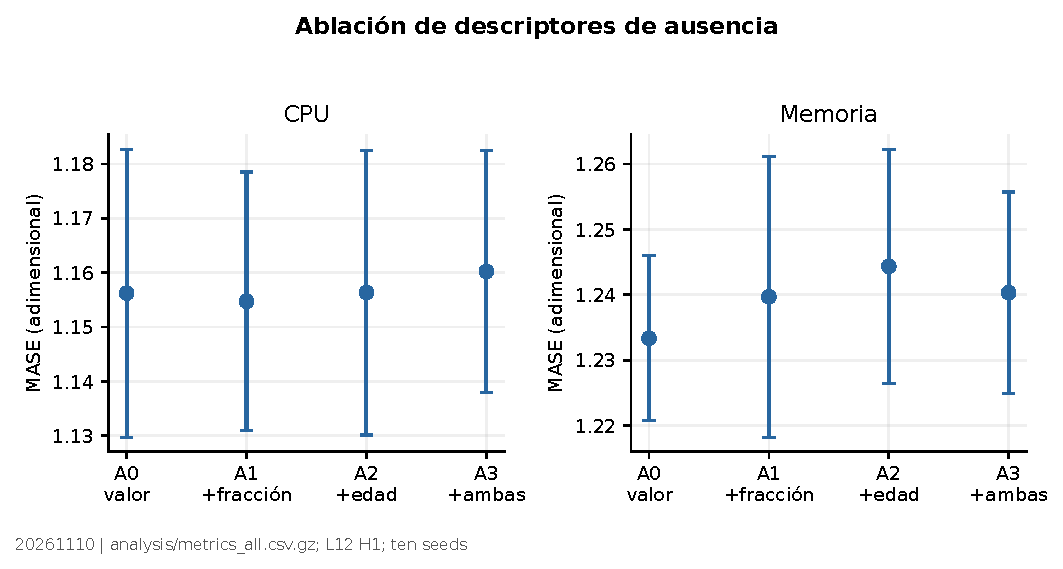
\includegraphics[width=0.79\textwidth]{figuras/es_11_ablations.pdf}
\caption{Medias A0--A3 y desviaciones entre diez medias de ajustes. Las barras son desviaciones descriptivas, no intervalos de confianza ni predictivos. Las familias se seleccionaron independientemente.}\label{fig:ablation}\end{figure*}
\begin{figure*}[!t]\centering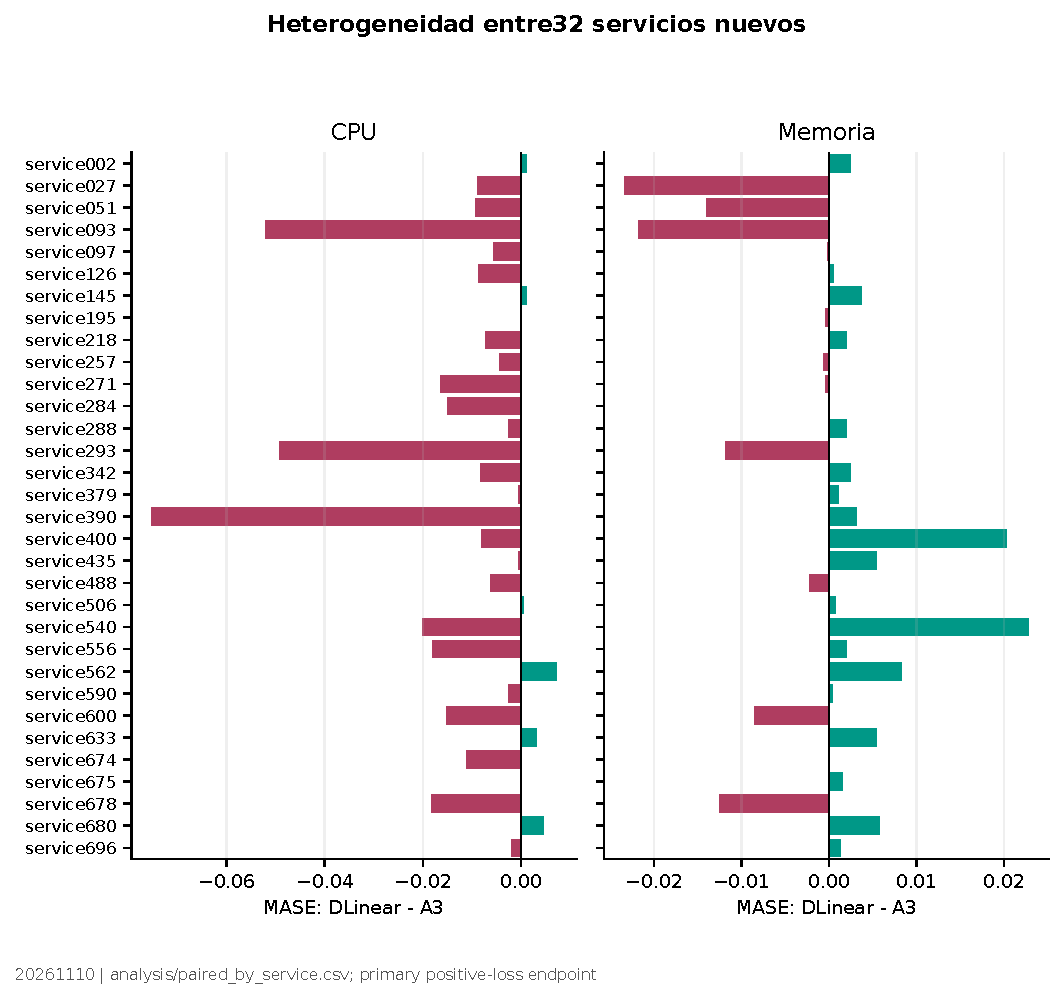
\includegraphics[width=0.71\textwidth]{figuras/es_15_services.pdf}
\caption{DLinear menos A3 por servicio, promediando semillas, máscaras y seis condiciones. Positivo favorece A3. Los servicios conectados son casos fijos, no muestras poblacionales independientes.}\label{fig:services}\end{figure*}
\begin{figure*}[!t]\centering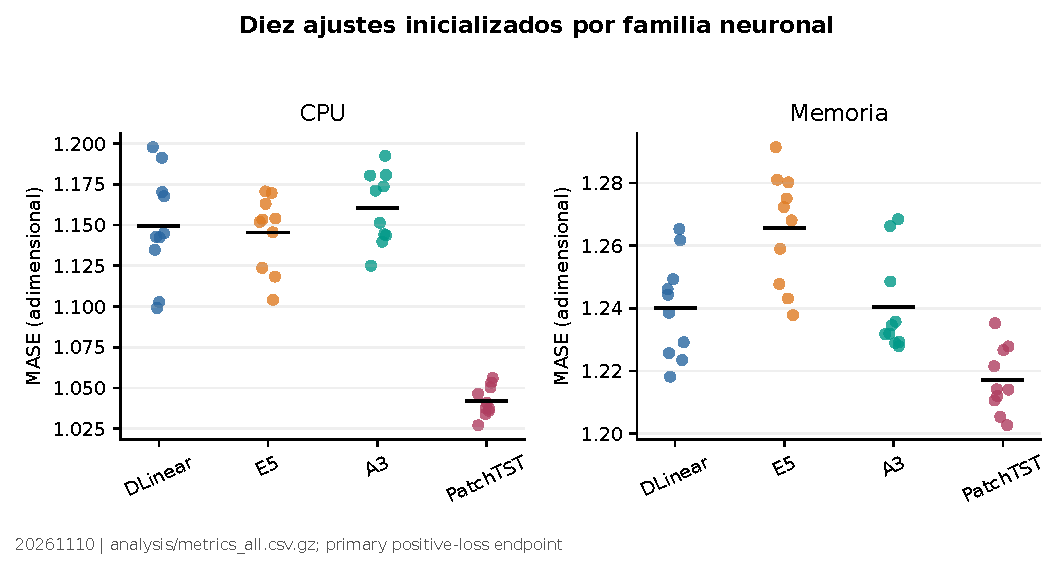
\includegraphics[width=0.76\textwidth]{figuras/es_10_seed_variability.pdf}
\caption{Diez medias por ajuste neuronal sobre servicios fijos, seis condiciones y veinte máscaras. Las marcas negras indican promedio; no son diez infraestructuras.}\label{fig:seeds}\end{figure*}

\subsection{Robustez frente a telemetría incompleta}
Las curvas de medias generalmente aumentan entre datos completos y 40\% de ausencia dispersa o por bloques cortos, Fig.~\ref{fig:loss}. No se afirma monotonía para cada servicio o máscara. A etiqueta 20\%, bloques prolongados fueron más difíciles que pérdidas correlacionadas para A3: CPU 1.2330 frente a 1.1342 y memoria 1.3743 frente a 1.1932. MAR no es una comparación controlada a 20\% porque realiza una fracción mayor. El suplemento retiene los tres mecanismos y todas las familias. Los ejemplos de máscaras muestran estructura espacial y duración impuestas, no fallas reales. Seleccionar una curva favorable no determina la conclusión.
\begin{figure*}[!t]\centering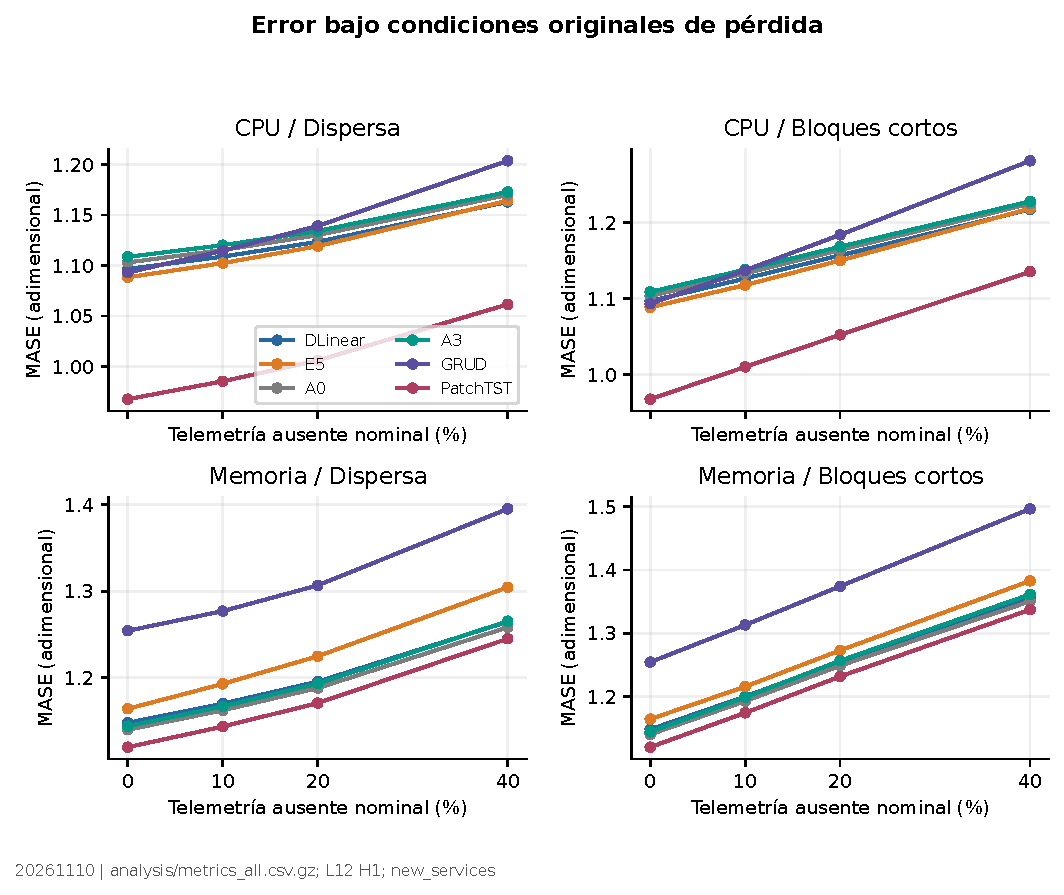
\includegraphics[width=0.76\textwidth]{figuras/es_07_loss.pdf}
\caption{MASE descriptivo bajo datos completos y pérdidas originales dispersas o por bloques. Las curvas seleccionadas facilitan lectura; las tablas y CSV conservan toda la comparación.}\label{fig:loss}\end{figure*}

\subsection{Horizontes directos y ventanas}
La comparación secundaria utiliza 1553 objetivos destino idénticos, filas 6452--8004, tres semillas, cinco máscaras y seis condiciones con pérdidas. A L12, CPU PatchTST aumenta de 1.0445 a treinta minutos a 1.6399 a seis horas; A3 pasa de 1.1584 a 1.9779. En memoria PatchTST pasa de 1.2264 a 2.1681 y A3 de 1.2436 a 2.3141. Cada horizonte ajusta un modelo directo; no son predicciones iteradas de un paso. Las historias más largas producen resultados mixtos: CPU A3 mejora de 1.1584 en L12 a 1.0966 en L48, pero memoria empeora de 1.2436 a 1.2560. PatchTST memoria tiene su menor valor de las tres historias en L24, 1.2190.

El punto H30 común difiere deliberadamente del principal completo y no lo sustituye. Las Figs.~\ref{fig:horizon} y~\ref{fig:history} y las Tablas~\ref{tab:horizon} y~\ref{tab:history} conservan el diseño estrella; no se ejecutaron todas las combinaciones de ventanas y horizontes. Una curva une observaciones ejecutadas sin demostrar interacciones factoriales ni significación confirmatoria.
\begin{figure*}[!t]\centering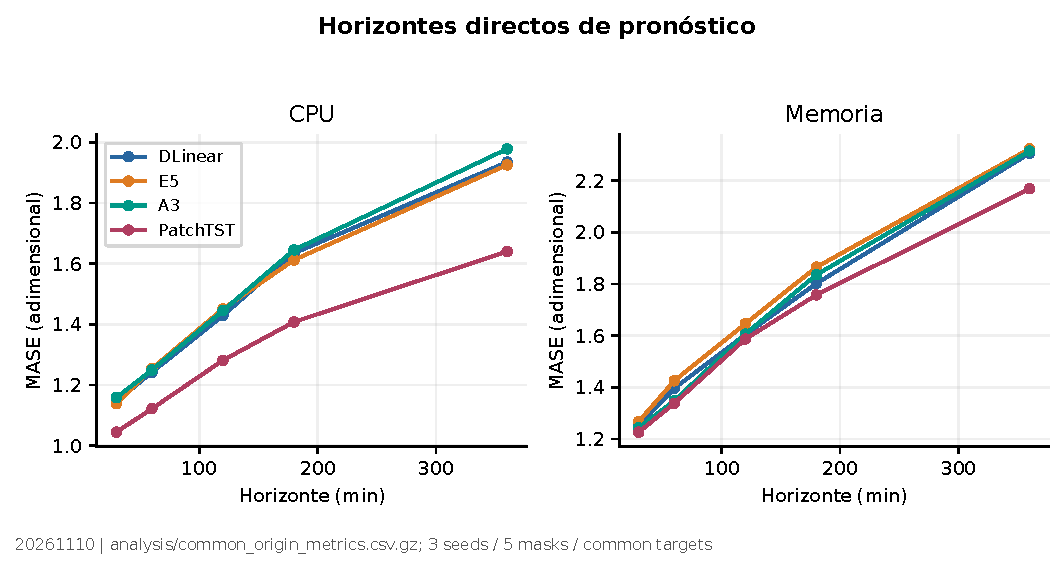
\includegraphics[width=0.79\textwidth]{figuras/es_08_horizon.pdf}
\caption{MASE con horizontes directos sobre 1553 objetivos comunes, tres semillas y cinco máscaras. Cada extremo usa pesos ajustados para ese horizonte.}\label{fig:horizon}\end{figure*}
\begin{figure*}[!t]\centering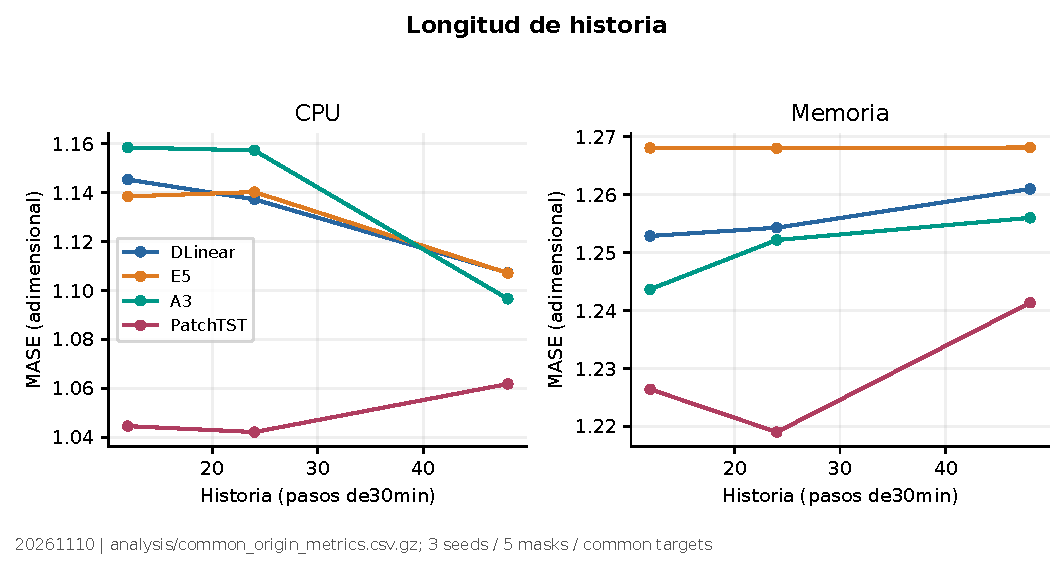
\includegraphics[width=0.79\textwidth]{figuras/es_09_history.pdf}
\caption{Sensibilidad a historia con horizonte treinta minutos y mismo soporte secundario. Las líneas son descriptivas.}\label{fig:history}\end{figure*}

\subsection{Transferencia externa a Alibaba}
En el día Alibaba, persistencia obtuvo el menor MASE de las catorce familias elegibles:2.3795 en CPU y 7.5150 en memoria normalizadas. A3 obtuvo 3.3593 y 9.9535; PatchTST 3.1112 y 10.5876. No se reajustó ningún método sobre los 36 intervalos objetivo. GRU de grafo se excluyó por ausencia de red externa. El denominador de seis horas y la diferencia entre medias de intervalos y muestras puntuales limitan la interpretación. Los errores absolutos de la Tabla~\ref{tab:external} son utilización normalizada, sin comparación directa con bytes o escala CPU ChronoGraph.

La Fig.~\ref{fig:external} conserva la inversión de clasificación: la mejor media primaria no se convierte en una ventaja universal entre dominios. Un día, 32 servicios elegidos por disponibilidad y 36 objetivos por servicio no sustentan validación externa concluyente. El volumen bruto de cientos de millones de filas documenta procesamiento, no tamaño efectivo independiente de evaluación.
\begin{figure*}[!t]\centering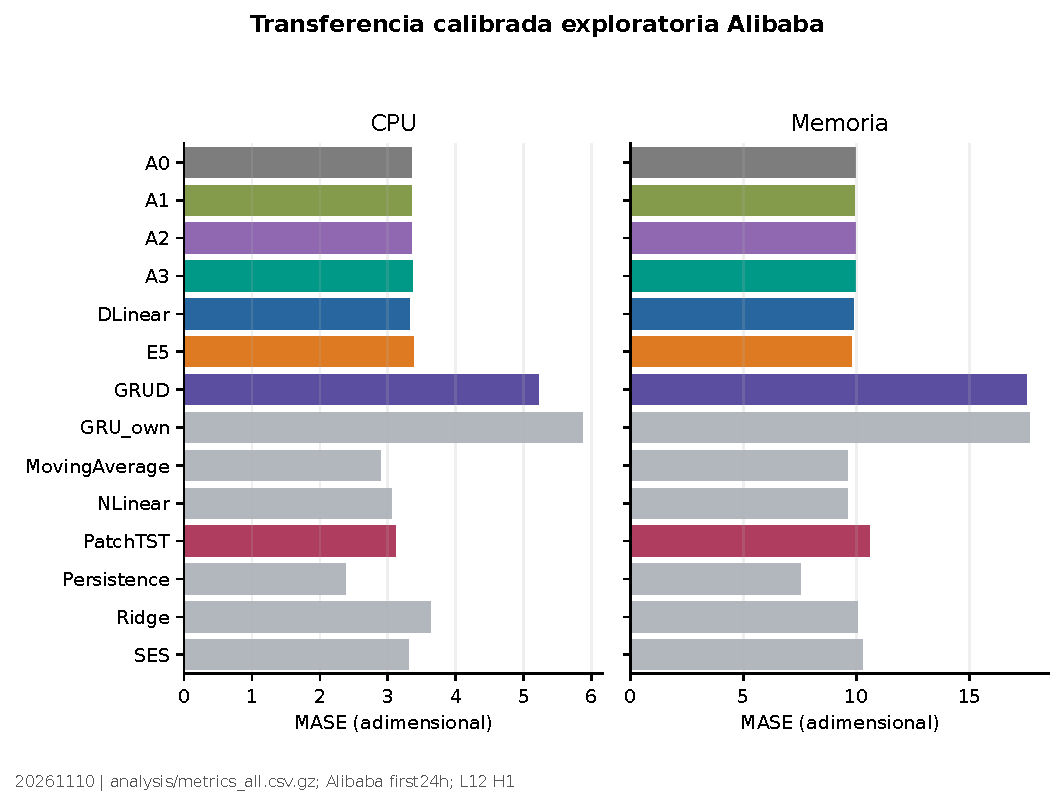
\includegraphics[width=0.79\textwidth]{figuras/es_12_external.pdf}
\caption{Transferencia exploratoria del primer día Alibaba:32 servicios, 36 objetivos semihorarios y seis horas de calibración. No representa replicación independiente entre infraestructuras.}\label{fig:external}\end{figure*}

\subsection{Coste computacional}\label{sec:cost}
A L12, A3 tiene 15 parámetros por recurso, DLinear 26 y E5 74. En B1/32 servicios, p 50 CPU fue 0.050~ms para A3, 0.057 para DLinear y 0.295 para E5; CUDA sincronizada 0.141, 0.281 y 0.665~ms. PatchTST tiene 2499 elementos entrenables y p 50 CPU 0.521~ms/CUDA1.212~ms. La Tabla~\ref{tab:efficiency} conserva p 95 y todas las familias. Son llamadas con tensores residentes, sin recolección, preparación o control. Algunos modelos compactos resultan más lentos en CUDA que CPU con este lote pequeño.

Las medianas de sumas de épocas completadas, incluyendo validación, fueron 8.56~s A3, 10.21 DLinear, 14.72 E5 y 42.88 PatchTST. Excluyen búsqueda, escritura de checkpoints e intentos incompletos fallidos. La Fig.~\ref{fig:latency} relaciona error con p 50 y la Fig.~\ref{fig:params} con tamaño. Las diferencias observadas no identifican una aceleración causal universal de hardware ni beneficios de SLA.
\begin{table*}[!t]
\caption{Elementos entrenables y p 50/p 95 en ms, B1/32 servicios. CUDA sincroniza ensayos y GRU-D usa reproducción sin coste inicial de captura. La suma de épocas es mediana de ajustes fuente, no duración total del proyecto.}\label{tab:efficiency}
\centering\footnotesize
\FitTable{\begin{tabular}{lrrrrrr}
\toprule
Modelo & Parámetros & CPU p50 & CPU p95 & CUDA p50 & CUDA p95 & Suma de épocas (s) \\
\midrule
Persistencia & 0 & 0.005 & 0.005 & 0.012 & 0.012 & sin medir \\
Media móvil & 0 & 0.014 & 0.015 & 0.023 & 0.025 & sin medir \\
Suavizamiento exponencial & 0 & 0.195 & 0.417 & 0.328 & 0.337 & sin medir \\
Ridge & 13 & 0.022 & 0.024 & 0.084 & 0.092 & sin medir \\
DLinear & 26 & 0.057 & 0.064 & 0.281 & 0.337 & 10.21 \\
NLinear & 13 & 0.031 & 0.045 & 0.095 & 0.102 & 7.62 \\
E5 & 74 & 0.295 & 0.317 & 0.665 & 0.681 & 14.72 \\
A0 & 13 & 0.022 & 0.023 & 0.085 & 0.095 & 7.26 \\
A1 & 14 & 0.046 & 0.049 & 0.125 & 0.134 & 7.99 \\
A2 & 14 & 0.030 & 0.032 & 0.104 & 0.116 & 7.10 \\
A3 & 15 & 0.050 & 0.056 & 0.141 & 0.166 & 8.56 \\
GRU (propia) & 841 & 0.425 & 0.450 & 0.341 & 0.360 & 15.41 \\
GRU (grafo) & 841 & 0.413 & 0.439 & 0.344 & 0.352 & 15.60 \\
GRU-D adaptada & 615 & 1.475 & 2.789 & 0.443 & 0.444 & 15.72 \\
PatchTST (pequeño) & 2499 & 0.521 & 0.546 & 1.212 & 1.316 & 42.88 \\
\bottomrule
\end{tabular}
}
\end{table*}
\begin{figure*}[!t]\centering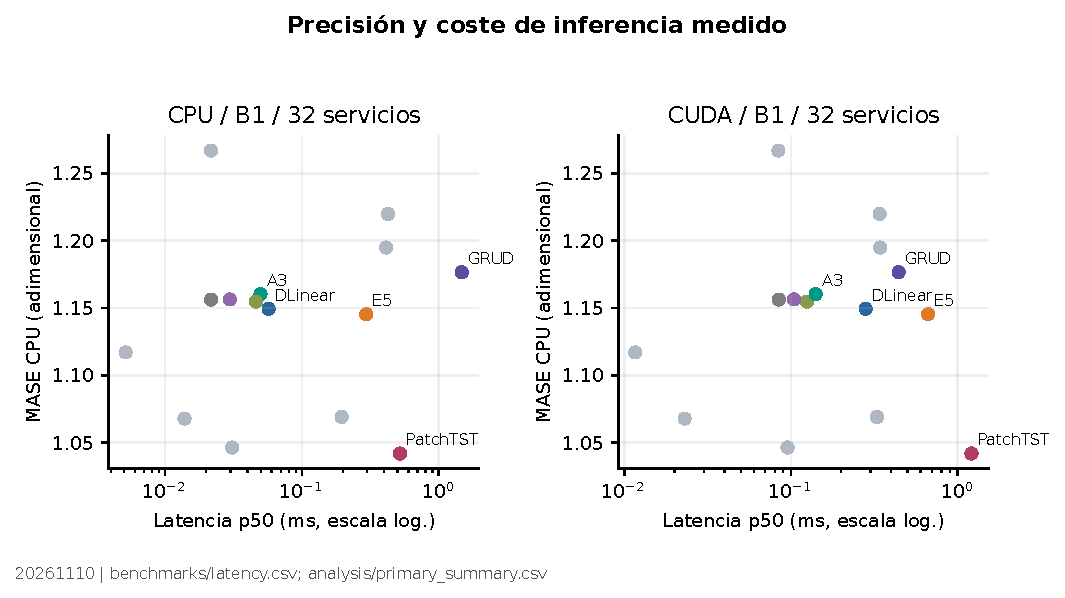
\includegraphics[width=0.79\textwidth]{figuras/es_13_latency.pdf}
\caption{MASE CPU y p 50 con entradas residentes. El equipo compartido y el alcance de la llamada limitan la interpretación operativa.}\label{fig:latency}\end{figure*}
\begin{figure*}[!t]\centering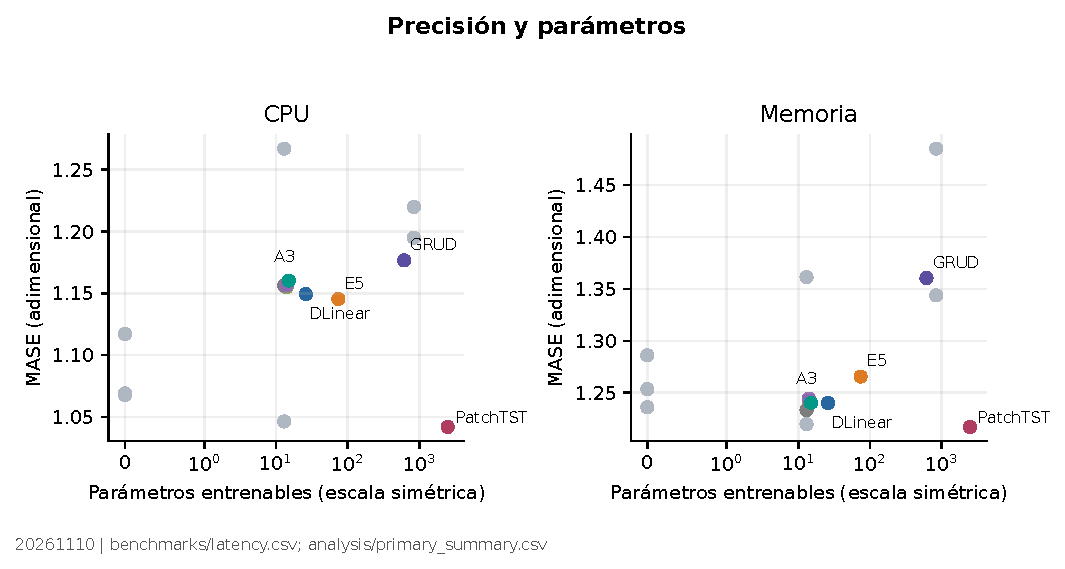
\includegraphics[width=0.79\textwidth]{figuras/es_14_parameters.pdf}
\caption{Error frente a parámetros entrenables. La escala logarítmica simétrica conserva referencias de cero parámetros. No incluye estados, calibración o coordinación.}\label{fig:params}\end{figure*}

El monitor muestreó RSS máximo del proceso 1725.47~MiB, sin capturar continuamente el pico. La RAM disponible del sistema se mantuvo sobre 10.87~GiB. La memoria GPU total alcanzó 3536~MiB y temperatura 75 gradosC; incluyen otras aplicaciones. El sensor CPU llegó a 92 gradosC y hubo un episodio de pausa del guardián. Se preservaron siete intentos GRU-D fallidos iniciales, 22 reintentos de entrenamiento por falta de memoria y 94 reducciones de lote de inferencia; todas las configuraciones finales tienen marcadores completos. No se midió energía del proyecto.

\subsection{Respuestas integradas a las preguntas}
La Tabla~\ref{tab:rq} conecta las fases sin promediar evidencia incompatible. La mejora histórica de memoria motiva una pregunta, sin sumarse a la ampliada para producir un efecto mayor. El volumen Alibaba no sustituye sus 36 objetivos. La auditoría verifica consistencia entre predicciones y métricas, no independencia de todo preprocesamiento desconocido del proveedor.
\begin{table*}[!t]
\caption{Respuestas basadas en evidencia. Las direcciones corresponden al experimento indicado y las cuatro pruebas principales se presentan por separado.}\label{tab:rq}
\centering\footnotesize
\begin{tabularx}{\linewidth}{p{.07\linewidth}XXX}
\toprule PI & Evidencia y dirección & Alcance & Límite \\\midrule
1 & Pérdidas originales elevan generalmente medias; bloques largos empeoran A3 & Trazas y mecanismos sintéticos & No prueba fallas reales ni todos los servicios \\
2 & E5 histórico mejora memoria y empeora CPU; DLinear fijo es afín & Parametrizaciones E/C/A separadas & Selección y optimización diferentes \\
3 & A3 no supera A0 agregado; descriptores E mixtos & Familias seleccionadas independientemente & No efecto causal ortogonal \\
4 & A3 usa 15 frente a 26/74; menor latencia medida & B1 residente CPU/CUDA medidos & Sin ventaja universal de precisión o energía \\
5 & PatchTST/NLinear menores medias principales; persistencia menor MASE externo & Destino 32 calibrado y un día Alibaba & Sin período independiente o validación poblacional \\
6 & Intervalos históricos cruzados amplios;A3/E5 memoria 10/10 & Datos y configuraciones fijos & Concentración por servicio y dependencia temporal \\
\bottomrule\end{tabularx}
\end{table*}
